\documentclass[tikz,border=5pt]{standalone}
\usepackage{amssymb}
\usepackage{amsfonts}
\usepackage{mathrsfs}
\usepackage{amsthm}
\usepackage{amsmath}
\usepackage{xcolor}
\usepackage{hyperref}
\usepackage{libertinus}
\usepackage{dsfont}
\usepackage{bm}
\usepackage{enumitem}
\usepackage{caption}
\usepackage{subcaption}
\usepackage{tikz}
\usepackage{quiver}

\newcommand{\R}{\mathbb{R}}
\newcommand{\C}{\mathbb{C}}
\newcommand{\N}{\mathbb{N}}
\newcommand{\Z}{\mathbb{Z}}
\newcommand{\Q}{\mathbb{Q}}

\newcommand{\id}{\operatorname{id}}

% differentials and derivatives
\renewcommand{\d}{\mathrm{d}}
\newcommand{\dd}{\,\d}
\newcommand{\pddf}[2]{\frac{\partial#1}{\partial#2}}
\newcommand{\ddt}{\frac{\d }{\d t}}
\newcommand{\ddtz}{\left.\ddt\right|_{t=0}}

\begin{document}
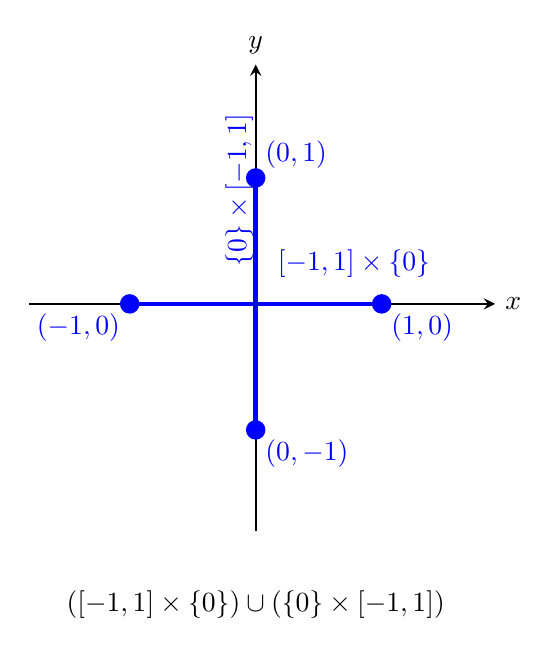
\begin{tikzpicture}[scale=1.6, >=stealth]

    % Axes
    \draw[->, thick] (-1.8,0) -- (1.9,0) node[right] {$x$};
    \draw[->, thick] (0,-1.8) -- (0,1.9) node[above] {$y$};

    % The cross: two closed unit segments crossing at the origin
    \draw[blue, ultra thick] (-1,0) -- (1,0);
    \draw[blue, ultra thick] (0,-1) -- (0,1);

    % The four endpoints belong to the set
    \fill[blue] (1,0) circle (2.2pt) node[anchor=north west] {$(1,0)$};
    \fill[blue] (-1,0) circle (2.2pt) node[anchor=north east] {$(-1,0)$};
    \fill[blue] (0,1) circle (2.2pt) node[anchor=south west] {$(0,1)$};
    \fill[blue] (0,-1) circle (2.2pt) node[anchor=north west] {$(0,-1)$};

    \node[blue, anchor=south] at (0.78,0.13) {$[-1,1]\times\{0\}$};
    \node[blue, anchor=west, rotate=90] at (-0.13,0.22) {$\{0\}\times[-1,1]$};

    \node[anchor=north] at (0,-2.2)
        {$([-1,1]\times\{0\})\cup(\{0\}\times[-1,1])$};

\end{tikzpicture}
\end{document}
